\documentclass[1p]{elsarticle_modified}
%\bibliographystyle{elsarticle-num}

%\usepackage[colorlinks]{hyperref}
%\usepackage{abbrmath_seonhwa} %\Abb, \Ascr, \Acal ,\Abf, \Afrak
\usepackage{amsfonts}
\usepackage{amssymb}
\usepackage{amsmath}
\usepackage{amsthm}
\usepackage{scalefnt}
\usepackage{amsbsy}
\usepackage{kotex}
\usepackage{caption}
\usepackage{subfig}
\usepackage{color}
\usepackage{graphicx}
\usepackage{xcolor} %% white, black, red, green, blue, cyan, magenta, yellow
\usepackage{float}
\usepackage{setspace}
\usepackage{hyperref}

\usepackage{tikz}
\usetikzlibrary{arrows}

\usepackage{multirow}
\usepackage{array} % fixed length table
\usepackage{hhline}

%%%%%%%%%%%%%%%%%%%%%
\makeatletter
\renewcommand*\env@matrix[1][\arraystretch]{%
	\edef\arraystretch{#1}%
	\hskip -\arraycolsep
	\let\@ifnextchar\new@ifnextchar
	\array{*\c@MaxMatrixCols c}}
\makeatother %https://tex.stackexchange.com/questions/14071/how-can-i-increase-the-line-spacing-in-a-matrix
%%%%%%%%%%%%%%%

\usepackage[normalem]{ulem}

\newcommand{\msout}[1]{\ifmmode\text{\sout{\ensuremath{#1}}}\else\sout{#1}\fi}
%SOURCE: \msout is \stkout macro in https://tex.stackexchange.com/questions/20609/strikeout-in-math-mode

\newcommand{\cancel}[1]{
	\ifmmode
	{\color{red}\msout{#1}}
	\else
	{\color{red}\sout{#1}}
	\fi
}

\newcommand{\add}[1]{
	{\color{blue}\uwave{#1}}
}

\newcommand{\replace}[2]{
	\ifmmode
	{\color{red}\msout{#1}}{\color{blue}\uwave{#2}}
	\else
	{\color{red}\sout{#1}}{\color{blue}\uwave{#2}}
	\fi
}

\newcommand{\Sol}{\mathcal{S}} %segment
\newcommand{\D}{D} %diagram
\newcommand{\A}{\mathcal{A}} %arc


%%%%%%%%%%%%%%%%%%%%%%%%%%%%%5 test

\def\sl{\operatorname{\textup{SL}}(2,\Cbb)}
\def\psl{\operatorname{\textup{PSL}}(2,\Cbb)}
\def\quan{\mkern 1mu \triangleright \mkern 1mu}

\theoremstyle{definition}
\newtheorem{thm}{Theorem}[section]
\newtheorem{prop}[thm]{Proposition}
\newtheorem{lem}[thm]{Lemma}
\newtheorem{ques}[thm]{Question}
\newtheorem{cor}[thm]{Corollary}
\newtheorem{defn}[thm]{Definition}
\newtheorem{exam}[thm]{Example}
\newtheorem{rmk}[thm]{Remark}
\newtheorem{alg}[thm]{Algorithm}

\newcommand{\I}{\sqrt{-1}}
\begin{document}

%\begin{frontmatter}
%
%\title{Boundary parabolic representations of knots up to 8 crossings}
%
%%% Group authors per affiliation:
%\author{Yunhi Cho} 
%\address{Department of Mathematics, University of Seoul, Seoul, Korea}
%\ead{yhcho@uos.ac.kr}
%
%
%\author{Seonhwa Kim} %\fnref{s_kim}}
%\address{Center for Geometry and Physics, Institute for Basic Science, Pohang, 37673, Korea}
%\ead{ryeona17@ibs.re.kr}
%
%\author{Hyuk Kim}
%\address{Department of Mathematical Sciences, Seoul National University, Seoul 08826, Korea}
%\ead{hyukkim@snu.ac.kr}
%
%\author{Seokbeom Yoon}
%\address{Department of Mathematical Sciences, Seoul National University, Seoul, 08826,  Korea}
%\ead{sbyoon15@snu.ac.kr}
%
%\begin{abstract}
%We find all boundary parabolic representation of knots up to 8 crossings.
%
%\end{abstract}
%\begin{keyword}
%    \MSC[2010] 57M25 
%\end{keyword}
%
%\end{frontmatter}

%\linenumbers
%\tableofcontents
%
\newcommand\colored[1]{\textcolor{white}{\rule[-0.35ex]{0.8em}{1.4ex}}\kern-0.8em\color{red} #1}%
%\newcommand\colored[1]{\textcolor{white}{ #1}\kern-2.17ex	\textcolor{white}{ #1}\kern-1.81ex	\textcolor{white}{ #1}\kern-2.15ex\color{red}#1	}

{\Large $\underline{11a_{92}~(K11a_{92})}$}

\setlength{\tabcolsep}{10pt}
\renewcommand{\arraystretch}{1.6}
\vspace{1cm}\begin{tabular}{m{100pt}>{\centering\arraybackslash}m{274pt}}
\multirow{5}{120pt}{
	\centering
	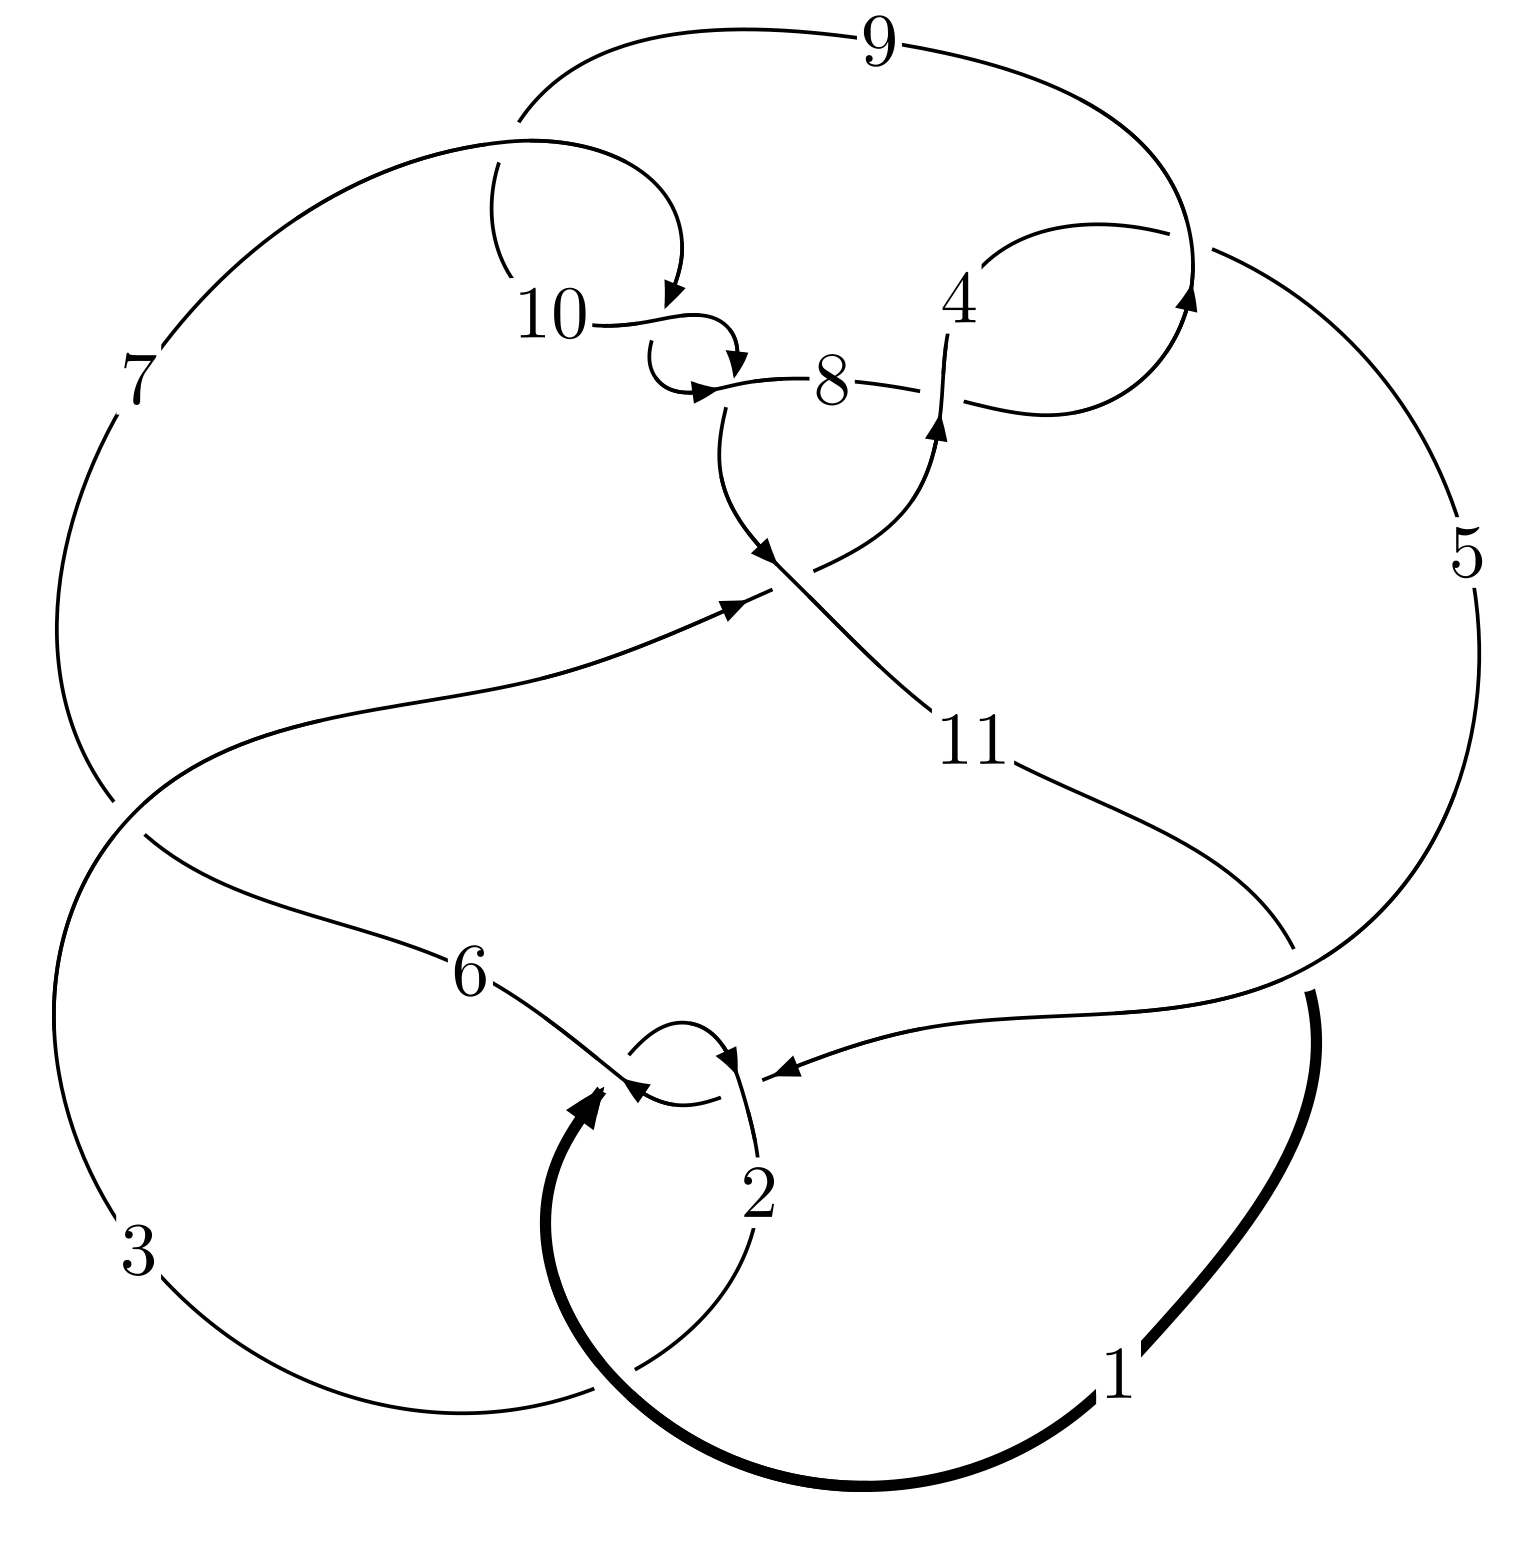
\includegraphics[width=112pt]{../../../GIT/diagram.site/Diagrams/png/341_11a_92.png}\\
\ \ \ A knot diagram\footnotemark}&
\allowdisplaybreaks
\textbf{Linearized knot diagam} \\
\cline{2-2}
 &
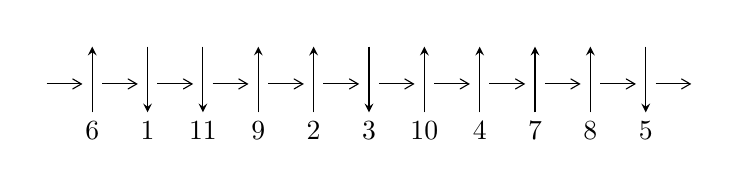
\begin{tikzpicture}[x=20pt, y=17pt]
	% nodes
	\node (C0) at (0, 0) {};
	\node (C1) at (1, 0) {};
	\node (C1U) at (1, +1) {};
	\node (C1D) at (1, -1) {6};

	\node (C2) at (2, 0) {};
	\node (C2U) at (2, +1) {};
	\node (C2D) at (2, -1) {1};

	\node (C3) at (3, 0) {};
	\node (C3U) at (3, +1) {};
	\node (C3D) at (3, -1) {11};

	\node (C4) at (4, 0) {};
	\node (C4U) at (4, +1) {};
	\node (C4D) at (4, -1) {9};

	\node (C5) at (5, 0) {};
	\node (C5U) at (5, +1) {};
	\node (C5D) at (5, -1) {2};

	\node (C6) at (6, 0) {};
	\node (C6U) at (6, +1) {};
	\node (C6D) at (6, -1) {3};

	\node (C7) at (7, 0) {};
	\node (C7U) at (7, +1) {};
	\node (C7D) at (7, -1) {10};

	\node (C8) at (8, 0) {};
	\node (C8U) at (8, +1) {};
	\node (C8D) at (8, -1) {4};

	\node (C9) at (9, 0) {};
	\node (C9U) at (9, +1) {};
	\node (C9D) at (9, -1) {7};

	\node (C10) at (10, 0) {};
	\node (C10U) at (10, +1) {};
	\node (C10D) at (10, -1) {8};

	\node (C11) at (11, 0) {};
	\node (C11U) at (11, +1) {};
	\node (C11D) at (11, -1) {5};
	\node (C12) at (12, 0) {};

	% arrows
	\draw[->,>={angle 60}]
	(C0) edge (C1) (C1) edge (C2) (C2) edge (C3) (C3) edge (C4) (C4) edge (C5) (C5) edge (C6) (C6) edge (C7) (C7) edge (C8) (C8) edge (C9) (C9) edge (C10) (C10) edge (C11) (C11) edge (C12) ;	\draw[->,>=stealth]
	(C1D) edge (C1U) (C2U) edge (C2D) (C3U) edge (C3D) (C4D) edge (C4U) (C5D) edge (C5U) (C6U) edge (C6D) (C7D) edge (C7U) (C8D) edge (C8U) (C9D) edge (C9U) (C10D) edge (C10U) (C11U) edge (C11D) ;
	\end{tikzpicture} \\
\hhline{~~} \\& 
\textbf{Solving Sequence} \\ \cline{2-2} 
 &
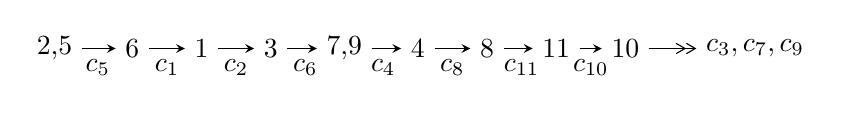
\begin{tikzpicture}[x=25pt, y=7pt]
	% node
	\node (A0) at (-1/8, 0) {2,5};
	\node (A1) at (1, 0) {6};
	\node (A2) at (2, 0) {1};
	\node (A3) at (3, 0) {3};
	\node (A4) at (65/16, 0) {7,9};
	\node (A5) at (41/8, 0) {4};
	\node (A6) at (49/8, 0) {8};
	\node (A7) at (57/8, 0) {11};
	\node (A8) at (65/8, 0) {10};
	\node (C1) at (1/2, -1) {$c_{5}$};
	\node (C2) at (3/2, -1) {$c_{1}$};
	\node (C3) at (5/2, -1) {$c_{2}$};
	\node (C4) at (7/2, -1) {$c_{6}$};
	\node (C5) at (37/8, -1) {$c_{4}$};
	\node (C6) at (45/8, -1) {$c_{8}$};
	\node (C7) at (53/8, -1) {$c_{11}$};
	\node (C8) at (61/8, -1) {$c_{10}$};
	\node (A9) at (10, 0) {$c_{3},c_{7},c_{9}$};

	% edge
	\draw[->,>=stealth]	
	(A0) edge (A1) (A1) edge (A2) (A2) edge (A3) (A3) edge (A4) (A4) edge (A5) (A5) edge (A6) (A6) edge (A7) (A7) edge (A8) ;
	\draw[->>,>={angle 60}]	
	(A8) edge (A9);
\end{tikzpicture} \\ 

\end{tabular} \\

\footnotetext{
The image of knot diagram is generated by the software ``\textbf{Draw programme}" developed by Andrew Bartholomew(\url{http://www.layer8.co.uk/maths/draw/index.htm\#Running-draw}), where we modified some parts for our purpose(\url{https://github.com/CATsTAILs/LinksPainter}).
}\phantom \\ \newline 
\centering \textbf{Ideals for irreducible components\footnotemark of $X_{\text{par}}$} 
 
\begin{align*}
I^u_{1}&=\langle 
u^{55}-2 u^{54}+\cdots+b+1,\;- u^{54}+u^{53}+\cdots+a+3,\;u^{56}-2 u^{55}+\cdots+5 u-1\rangle \\
I^u_{2}&=\langle 
b,\;- u^2+a- u-1,\;u^5+u^4+2 u^3+u^2+u+1\rangle \\
\\
\end{align*}
\raggedright * 2 irreducible components of $\dim_{\mathbb{C}}=0$, with total 61 representations.\\
\footnotetext{All coefficients of polynomials are rational numbers. But the coefficients are sometimes approximated in decimal forms when there is not enough margin.}
\newpage
\renewcommand{\arraystretch}{1}
\centering \section*{I. $I^u_{1}= \langle u^{55}-2 u^{54}+\cdots+b+1,\;- u^{54}+u^{53}+\cdots+a+3,\;u^{56}-2 u^{55}+\cdots+5 u-1 \rangle$}
\flushleft \textbf{(i) Arc colorings}\\
\begin{tabular}{m{7pt} m{180pt} m{7pt} m{180pt} }
\flushright $a_{2}=$&$\begin{pmatrix}0\\u\end{pmatrix}$ \\
\flushright $a_{5}=$&$\begin{pmatrix}1\\0\end{pmatrix}$ \\
\flushright $a_{6}=$&$\begin{pmatrix}1\\- u^2\end{pmatrix}$ \\
\flushright $a_{1}=$&$\begin{pmatrix}- u\\u^3+u\end{pmatrix}$ \\
\flushright $a_{3}=$&$\begin{pmatrix}- u^3\\u^5+u^3+u\end{pmatrix}$ \\
\flushright $a_{7}=$&$\begin{pmatrix}- u^6- u^4+1\\u^8+2 u^6+2 u^4\end{pmatrix}$ \\
\flushright $a_{9}=$&$\begin{pmatrix}u^{54}- u^{53}+\cdots+6 u-3\\- u^{55}+2 u^{54}+\cdots+6 u-1\end{pmatrix}$ \\
\flushright $a_{4}=$&$\begin{pmatrix}- u^{11}-2 u^9-2 u^7- u^3\\- u^{11}-3 u^9-4 u^7- u^5+u^3+u\end{pmatrix}$ \\
\flushright $a_{8}=$&$\begin{pmatrix}- u^{54}+u^{53}+\cdots+u-2\\u^{55}-2 u^{54}+\cdots-3 u+1\end{pmatrix}$ \\
\flushright $a_{11}=$&$\begin{pmatrix}u^3\\u^3+u\end{pmatrix}$ \\
\flushright $a_{10}=$&$\begin{pmatrix}- u^{51}+u^{50}+\cdots+4 u-2\\u^{30}+8 u^{28}+\cdots- u^2+2 u\end{pmatrix}$\\ \flushright $a_{10}=$&$\begin{pmatrix}- u^{51}+u^{50}+\cdots+4 u-2\\u^{30}+8 u^{28}+\cdots- u^2+2 u\end{pmatrix}$\\&\end{tabular}
\flushleft \textbf{(ii) Obstruction class $= -1$}\\~\\
\flushleft \textbf{(iii) Cusp Shapes $= 4 u^{55}-11 u^{54}+\cdots-30 u+15$}\\~\\
\newpage\renewcommand{\arraystretch}{1}
\flushleft \textbf{(iv) u-Polynomials at the component}\newline \\
\begin{tabular}{m{50pt}|m{274pt}}
Crossings & \hspace{64pt}u-Polynomials at each crossing \\
\hline $$\begin{aligned}c_{1},c_{5}\end{aligned}$$&$\begin{aligned}
&u^{56}-2 u^{55}+\cdots+5 u-1
\end{aligned}$\\
\hline $$\begin{aligned}c_{2}\end{aligned}$$&$\begin{aligned}
&u^{56}+30 u^{55}+\cdots-5 u+1
\end{aligned}$\\
\hline $$\begin{aligned}c_{3}\end{aligned}$$&$\begin{aligned}
&u^{56}-6 u^{55}+\cdots+2207 u+61
\end{aligned}$\\
\hline $$\begin{aligned}c_{4},c_{8}\end{aligned}$$&$\begin{aligned}
&u^{56}+u^{55}+\cdots-72 u^2+32
\end{aligned}$\\
\hline $$\begin{aligned}c_{6},c_{11}\end{aligned}$$&$\begin{aligned}
&u^{56}+2 u^{55}+\cdots-117 u-17
\end{aligned}$\\
\hline $$\begin{aligned}c_{7},c_{9},c_{10}\end{aligned}$$&$\begin{aligned}
&u^{56}+6 u^{55}+\cdots-5 u-1
\end{aligned}$\\
\hline
\end{tabular}\\~\\
\newpage\renewcommand{\arraystretch}{1}
\flushleft \textbf{(v) Riley Polynomials at the component}\newline \\
\begin{tabular}{m{50pt}|m{274pt}}
Crossings & \hspace{64pt}Riley Polynomials at each crossing \\
\hline $$\begin{aligned}c_{1},c_{5}\end{aligned}$$&$\begin{aligned}
&y^{56}+30 y^{55}+\cdots-5 y+1
\end{aligned}$\\
\hline $$\begin{aligned}c_{2}\end{aligned}$$&$\begin{aligned}
&y^{56}-6 y^{55}+\cdots-93 y+1
\end{aligned}$\\
\hline $$\begin{aligned}c_{3}\end{aligned}$$&$\begin{aligned}
&y^{56}+18 y^{55}+\cdots-3978053 y+3721
\end{aligned}$\\
\hline $$\begin{aligned}c_{4},c_{8}\end{aligned}$$&$\begin{aligned}
&y^{56}-33 y^{55}+\cdots-4608 y+1024
\end{aligned}$\\
\hline $$\begin{aligned}c_{6},c_{11}\end{aligned}$$&$\begin{aligned}
&y^{56}-42 y^{55}+\cdots-3965 y+289
\end{aligned}$\\
\hline $$\begin{aligned}c_{7},c_{9},c_{10}\end{aligned}$$&$\begin{aligned}
&y^{56}-54 y^{55}+\cdots-15 y+1
\end{aligned}$\\
\hline
\end{tabular}\\~\\
\newpage\flushleft \textbf{(vi) Complex Volumes and Cusp Shapes}
$$\begin{array}{c|c|c}  
\text{Solutions to }I^u_{1}& \I (\text{vol} + \sqrt{-1}CS) & \text{Cusp shape}\\
 \hline 
\begin{aligned}
u &= -0.541939 + 0.811305 I \\
a &= \phantom{-}1.42851 + 1.45771 I \\
b &= -1.123670 + 0.266261 I\end{aligned}
 & \phantom{-}2.81877 - 4.58854 I & \phantom{-}7.32192 + 7.37069 I \\ \hline\begin{aligned}
u &= -0.541939 - 0.811305 I \\
a &= \phantom{-}1.42851 - 1.45771 I \\
b &= -1.123670 - 0.266261 I\end{aligned}
 & \phantom{-}2.81877 + 4.58854 I & \phantom{-}7.32192 - 7.37069 I \\ \hline\begin{aligned}
u &= -0.593449 + 0.851697 I \\
a &= -1.01997 - 1.80907 I \\
b &= \phantom{-}1.38769 - 0.52689 I\end{aligned}
 & \phantom{-}9.36273 - 8.19631 I & \phantom{-}9.19540 + 7.01031 I \\ \hline\begin{aligned}
u &= -0.593449 - 0.851697 I \\
a &= -1.01997 + 1.80907 I \\
b &= \phantom{-}1.38769 + 0.52689 I\end{aligned}
 & \phantom{-}9.36273 + 8.19631 I & \phantom{-}9.19540 - 7.01031 I \\ \hline\begin{aligned}
u &= \phantom{-}0.546314 + 0.769644 I \\
a &= \phantom{-}0.992511 - 0.378537 I \\
b &= \phantom{-}0.058951 - 1.153390 I\end{aligned}
 & \phantom{-}5.03153 + 2.19878 I & \phantom{-}8.69192 - 3.70981 I \\ \hline\begin{aligned}
u &= \phantom{-}0.546314 - 0.769644 I \\
a &= \phantom{-}0.992511 + 0.378537 I \\
b &= \phantom{-}0.058951 + 1.153390 I\end{aligned}
 & \phantom{-}5.03153 - 2.19878 I & \phantom{-}8.69192 + 3.70981 I \\ \hline\begin{aligned}
u &= \phantom{-}0.128995 + 0.928935 I \\
a &= -0.49469 - 1.36046 I \\
b &= -0.698724 - 0.392096 I\end{aligned}
 & -1.44134 + 1.72632 I & -2.72624 - 5.24259 I \\ \hline\begin{aligned}
u &= \phantom{-}0.128995 - 0.928935 I \\
a &= -0.49469 + 1.36046 I \\
b &= -0.698724 + 0.392096 I\end{aligned}
 & -1.44134 - 1.72632 I & -2.72624 + 5.24259 I \\ \hline\begin{aligned}
u &= -0.618401 + 0.677884 I \\
a &= \phantom{-}0.634942 + 0.465765 I \\
b &= -1.39776 - 0.45849 I\end{aligned}
 & \phantom{-}9.85976 + 3.46157 I & \phantom{-}10.53207 - 0.66652 I \\ \hline\begin{aligned}
u &= -0.618401 - 0.677884 I \\
a &= \phantom{-}0.634942 - 0.465765 I \\
b &= -1.39776 + 0.45849 I\end{aligned}
 & \phantom{-}9.85976 - 3.46157 I & \phantom{-}10.53207 + 0.66652 I\\
 \hline 
 \end{array}$$\newpage$$\begin{array}{c|c|c}  
\text{Solutions to }I^u_{1}& \I (\text{vol} + \sqrt{-1}CS) & \text{Cusp shape}\\
 \hline 
\begin{aligned}
u &= -0.536957 + 0.721498 I \\
a &= -1.33171 - 0.63904 I \\
b &= \phantom{-}1.094330 + 0.157058 I\end{aligned}
 & \phantom{-}3.07741 + 0.22694 I & \phantom{-}8.69395 - 0.01547 I \\ \hline\begin{aligned}
u &= -0.536957 - 0.721498 I \\
a &= -1.33171 + 0.63904 I \\
b &= \phantom{-}1.094330 - 0.157058 I\end{aligned}
 & \phantom{-}3.07741 - 0.22694 I & \phantom{-}8.69395 + 0.01547 I \\ \hline\begin{aligned}
u &= \phantom{-}0.393541 + 0.806213 I \\
a &= -0.534427 + 0.136082 I \\
b &= -0.100768 + 0.460978 I\end{aligned}
 & -0.09593 + 1.71111 I & -0.21296 - 4.36138 I \\ \hline\begin{aligned}
u &= \phantom{-}0.393541 - 0.806213 I \\
a &= -0.534427 - 0.136082 I \\
b &= -0.100768 - 0.460978 I\end{aligned}
 & -0.09593 - 1.71111 I & -0.21296 + 4.36138 I \\ \hline\begin{aligned}
u &= \phantom{-}0.165097 + 1.107340 I \\
a &= \phantom{-}1.56163 + 1.18520 I \\
b &= \phantom{-}1.222870 + 0.358512 I\end{aligned}
 & \phantom{-}3.95584 + 4.04331 I & \phantom{-}3.44250 - 3.73640 I \\ \hline\begin{aligned}
u &= \phantom{-}0.165097 - 1.107340 I \\
a &= \phantom{-}1.56163 - 1.18520 I \\
b &= \phantom{-}1.222870 - 0.358512 I\end{aligned}
 & \phantom{-}3.95584 - 4.04331 I & \phantom{-}3.44250 + 3.73640 I \\ \hline\begin{aligned}
u &= \phantom{-}0.819442 + 0.178280 I \\
a &= -0.357670 - 1.253280 I \\
b &= \phantom{-}1.31600 - 0.63627 I\end{aligned}
 & \phantom{-}5.92889 - 9.27747 I & \phantom{-}7.55643 + 5.32356 I \\ \hline\begin{aligned}
u &= \phantom{-}0.819442 - 0.178280 I \\
a &= -0.357670 + 1.253280 I \\
b &= \phantom{-}1.31600 + 0.63627 I\end{aligned}
 & \phantom{-}5.92889 + 9.27747 I & \phantom{-}7.55643 - 5.32356 I \\ \hline\begin{aligned}
u &= -0.837877\phantom{ +0.000000I} \\
a &= \phantom{-}0.756831\phantom{ +0.000000I} \\
b &= \phantom{-}0.948658\phantom{ +0.000000I}\end{aligned}
 & \phantom{-}0.628307\phantom{ +0.000000I} & \phantom{-}8.59010\phantom{ +0.000000I} \\ \hline\begin{aligned}
u &= \phantom{-}0.775248 + 0.160784 I \\
a &= \phantom{-}0.738440 + 1.157850 I \\
b &= -1.121220 + 0.448045 I\end{aligned}
 & -0.03936 - 5.21507 I & \phantom{-}4.57400 + 5.37582 I\\
 \hline 
 \end{array}$$\newpage$$\begin{array}{c|c|c}  
\text{Solutions to }I^u_{1}& \I (\text{vol} + \sqrt{-1}CS) & \text{Cusp shape}\\
 \hline 
\begin{aligned}
u &= \phantom{-}0.775248 - 0.160784 I \\
a &= \phantom{-}0.738440 - 1.157850 I \\
b &= -1.121220 - 0.448045 I\end{aligned}
 & -0.03936 + 5.21507 I & \phantom{-}4.57400 - 5.37582 I \\ \hline\begin{aligned}
u &= \phantom{-}0.527916 + 1.093820 I \\
a &= \phantom{-}0.85567 + 1.31151 I \\
b &= \phantom{-}1.41225 - 0.21941 I\end{aligned}
 & \phantom{-}6.18656 + 2.95129 I & \phantom{-0.000000 } 0 \\ \hline\begin{aligned}
u &= \phantom{-}0.527916 - 1.093820 I \\
a &= \phantom{-}0.85567 - 1.31151 I \\
b &= \phantom{-}1.41225 + 0.21941 I\end{aligned}
 & \phantom{-}6.18656 - 2.95129 I & \phantom{-0.000000 } 0 \\ \hline\begin{aligned}
u &= \phantom{-}0.406423 + 1.148900 I \\
a &= -0.206924 + 0.240072 I \\
b &= -0.945829 + 0.294251 I\end{aligned}
 & -2.27409 + 3.17603 I & \phantom{-0.000000 } 0 \\ \hline\begin{aligned}
u &= \phantom{-}0.406423 - 1.148900 I \\
a &= -0.206924 - 0.240072 I \\
b &= -0.945829 - 0.294251 I\end{aligned}
 & -2.27409 - 3.17603 I & \phantom{-0.000000 } 0 \\ \hline\begin{aligned}
u &= -0.373696 + 1.162320 I \\
a &= \phantom{-}0.11056 + 2.44091 I \\
b &= -0.376968 + 1.039610 I\end{aligned}
 & -1.226340 - 0.673936 I & \phantom{-0.000000 } 0 \\ \hline\begin{aligned}
u &= -0.373696 - 1.162320 I \\
a &= \phantom{-}0.11056 - 2.44091 I \\
b &= -0.376968 - 1.039610 I\end{aligned}
 & -1.226340 + 0.673936 I & \phantom{-0.000000 } 0 \\ \hline\begin{aligned}
u &= \phantom{-}0.696924 + 0.334113 I \\
a &= \phantom{-}0.495506 + 0.067097 I \\
b &= -1.378520 - 0.306067 I\end{aligned}
 & \phantom{-}8.39220 + 1.73145 I & \phantom{-}10.27072 - 1.13053 I \\ \hline\begin{aligned}
u &= \phantom{-}0.696924 - 0.334113 I \\
a &= \phantom{-}0.495506 - 0.067097 I \\
b &= -1.378520 + 0.306067 I\end{aligned}
 & \phantom{-}8.39220 - 1.73145 I & \phantom{-}10.27072 + 1.13053 I \\ \hline\begin{aligned}
u &= -0.741697 + 0.174610 I \\
a &= \phantom{-}0.470285 - 0.832398 I \\
b &= \phantom{-}0.280634 - 1.119790 I\end{aligned}
 & \phantom{-}2.61340 + 2.94506 I & \phantom{-}6.64873 - 2.47914 I\\
 \hline 
 \end{array}$$\newpage$$\begin{array}{c|c|c}  
\text{Solutions to }I^u_{1}& \I (\text{vol} + \sqrt{-1}CS) & \text{Cusp shape}\\
 \hline 
\begin{aligned}
u &= -0.741697 - 0.174610 I \\
a &= \phantom{-}0.470285 + 0.832398 I \\
b &= \phantom{-}0.280634 + 1.119790 I\end{aligned}
 & \phantom{-}2.61340 - 2.94506 I & \phantom{-}6.64873 + 2.47914 I \\ \hline\begin{aligned}
u &= -0.126536 + 0.746458 I \\
a &= -0.84177 + 2.11295 I \\
b &= \phantom{-}0.411324 + 0.477215 I\end{aligned}
 & \phantom{-}1.064190 - 0.808693 I & \phantom{-}2.55500 - 2.42625 I \\ \hline\begin{aligned}
u &= -0.126536 - 0.746458 I \\
a &= -0.84177 - 2.11295 I \\
b &= \phantom{-}0.411324 - 0.477215 I\end{aligned}
 & \phantom{-}1.064190 + 0.808693 I & \phantom{-}2.55500 + 2.42625 I \\ \hline\begin{aligned}
u &= \phantom{-}0.369831 + 1.188440 I \\
a &= \phantom{-}0.956977 - 0.911104 I \\
b &= \phantom{-}1.068040 - 0.502274 I\end{aligned}
 & -4.02517 - 1.42731 I & \phantom{-0.000000 } 0 \\ \hline\begin{aligned}
u &= \phantom{-}0.369831 - 1.188440 I \\
a &= \phantom{-}0.956977 + 0.911104 I \\
b &= \phantom{-}1.068040 + 0.502274 I\end{aligned}
 & -4.02517 + 1.42731 I & \phantom{-0.000000 } 0 \\ \hline\begin{aligned}
u &= -0.749356 + 0.064381 I \\
a &= -0.349458 + 0.536326 I \\
b &= -0.335252 + 0.643104 I\end{aligned}
 & -2.43135 + 0.93671 I & -0.980703 - 0.861698 I \\ \hline\begin{aligned}
u &= -0.749356 - 0.064381 I \\
a &= -0.349458 - 0.536326 I \\
b &= -0.335252 - 0.643104 I\end{aligned}
 & -2.43135 - 0.93671 I & -0.980703 + 0.861698 I \\ \hline\begin{aligned}
u &= \phantom{-}0.495429 + 1.155840 I \\
a &= \phantom{-}0.25566 - 1.70729 I \\
b &= -1.092030 - 0.173225 I\end{aligned}
 & -1.62056 + 4.94124 I & \phantom{-0.000000 } 0 \\ \hline\begin{aligned}
u &= \phantom{-}0.495429 - 1.155840 I \\
a &= \phantom{-}0.25566 + 1.70729 I \\
b &= -1.092030 + 0.173225 I\end{aligned}
 & -1.62056 - 4.94124 I & \phantom{-0.000000 } 0 \\ \hline\begin{aligned}
u &= -0.424253 + 1.189480 I \\
a &= \phantom{-}0.12864 - 1.60526 I \\
b &= \phantom{-}0.405838 - 0.694649 I\end{aligned}
 & -6.03353 - 3.18510 I & \phantom{-0.000000 } 0\\
 \hline 
 \end{array}$$\newpage$$\begin{array}{c|c|c}  
\text{Solutions to }I^u_{1}& \I (\text{vol} + \sqrt{-1}CS) & \text{Cusp shape}\\
 \hline 
\begin{aligned}
u &= -0.424253 - 1.189480 I \\
a &= \phantom{-}0.12864 + 1.60526 I \\
b &= \phantom{-}0.405838 + 0.694649 I\end{aligned}
 & -6.03353 + 3.18510 I & \phantom{-0.000000 } 0 \\ \hline\begin{aligned}
u &= \phantom{-}0.347664 + 1.216700 I \\
a &= -1.59497 + 1.08012 I \\
b &= -1.263120 + 0.629980 I\end{aligned}
 & \phantom{-}1.65628 - 5.42117 I & \phantom{-0.000000 } 0 \\ \hline\begin{aligned}
u &= \phantom{-}0.347664 - 1.216700 I \\
a &= -1.59497 - 1.08012 I \\
b &= -1.263120 - 0.629980 I\end{aligned}
 & \phantom{-}1.65628 + 5.42117 I & \phantom{-0.000000 } 0 \\ \hline\begin{aligned}
u &= -0.509728 + 1.166280 I \\
a &= -1.69077 - 1.44666 I \\
b &= -0.328834 - 1.173990 I\end{aligned}
 & -0.26647 - 7.63409 I & \phantom{-0.000000 } 0 \\ \hline\begin{aligned}
u &= -0.509728 - 1.166280 I \\
a &= -1.69077 + 1.44666 I \\
b &= -0.328834 + 1.173990 I\end{aligned}
 & -0.26647 + 7.63409 I & \phantom{-0.000000 } 0 \\ \hline\begin{aligned}
u &= -0.476321 + 1.185870 I \\
a &= \phantom{-}1.13864 + 0.86802 I \\
b &= \phantom{-}0.294208 + 0.702336 I\end{aligned}
 & -5.66376 - 5.43442 I & \phantom{-0.000000 } 0 \\ \hline\begin{aligned}
u &= -0.476321 - 1.185870 I \\
a &= \phantom{-}1.13864 - 0.86802 I \\
b &= \phantom{-}0.294208 - 0.702336 I\end{aligned}
 & -5.66376 + 5.43442 I & \phantom{-0.000000 } 0 \\ \hline\begin{aligned}
u &= \phantom{-}0.513303 + 1.179050 I \\
a &= -0.19445 + 2.45753 I \\
b &= \phantom{-}1.158800 + 0.479620 I\end{aligned}
 & -3.01871 + 9.99320 I & \phantom{-0.000000 } 0 \\ \hline\begin{aligned}
u &= \phantom{-}0.513303 - 1.179050 I \\
a &= -0.19445 - 2.45753 I \\
b &= \phantom{-}1.158800 - 0.479620 I\end{aligned}
 & -3.01871 - 9.99320 I & \phantom{-0.000000 } 0 \\ \hline\begin{aligned}
u &= \phantom{-}0.680569 + 0.163703 I \\
a &= -1.128560 - 0.586189 I \\
b &= \phantom{-}0.997782 - 0.105266 I\end{aligned}
 & \phantom{-}1.216130 - 0.445746 I & \phantom{-}7.76853 + 0.07614 I\\
 \hline 
 \end{array}$$\newpage$$\begin{array}{c|c|c}  
\text{Solutions to }I^u_{1}& \I (\text{vol} + \sqrt{-1}CS) & \text{Cusp shape}\\
 \hline 
\begin{aligned}
u &= \phantom{-}0.680569 - 0.163703 I \\
a &= -1.128560 + 0.586189 I \\
b &= \phantom{-}0.997782 + 0.105266 I\end{aligned}
 & \phantom{-}1.216130 + 0.445746 I & \phantom{-}7.76853 - 0.07614 I \\ \hline\begin{aligned}
u &= \phantom{-}0.529749 + 1.189840 I \\
a &= -0.08999 - 2.82061 I \\
b &= -1.31987 - 0.67018 I\end{aligned}
 & \phantom{-}2.9322 + 14.2422 I & \phantom{-0.000000 } 0 \\ \hline\begin{aligned}
u &= \phantom{-}0.529749 - 1.189840 I \\
a &= -0.08999 + 2.82061 I \\
b &= -1.31987 + 0.67018 I\end{aligned}
 & \phantom{-}2.9322 - 14.2422 I & \phantom{-0.000000 } 0 \\ \hline\begin{aligned}
u &= -0.455869 + 1.229250 I \\
a &= -1.46012 + 0.80106 I \\
b &= -0.906346 + 0.052067 I\end{aligned}
 & -3.05418 - 4.60578 I & \phantom{-0.000000 } 0 \\ \hline\begin{aligned}
u &= -0.455869 - 1.229250 I \\
a &= -1.46012 - 0.80106 I \\
b &= -0.906346 - 0.052067 I\end{aligned}
 & -3.05418 + 4.60578 I & \phantom{-0.000000 } 0 \\ \hline\begin{aligned}
u &= \phantom{-}0.341383\phantom{ +0.000000I} \\
a &= -1.70182\phantom{ +0.000000I} \\
b &= \phantom{-}0.611698\phantom{ +0.000000I}\end{aligned}
 & \phantom{-}1.00387\phantom{ +0.000000I} & \phantom{-}10.1330\phantom{ +0.000000I}\\
 \hline 
 \end{array}$$\newpage\newpage\renewcommand{\arraystretch}{1}
\centering \section*{II. $I^u_{2}= \langle b,\;- u^2+a- u-1,\;u^5+u^4+2 u^3+u^2+u+1 \rangle$}
\flushleft \textbf{(i) Arc colorings}\\
\begin{tabular}{m{7pt} m{180pt} m{7pt} m{180pt} }
\flushright $a_{2}=$&$\begin{pmatrix}0\\u\end{pmatrix}$ \\
\flushright $a_{5}=$&$\begin{pmatrix}1\\0\end{pmatrix}$ \\
\flushright $a_{6}=$&$\begin{pmatrix}1\\- u^2\end{pmatrix}$ \\
\flushright $a_{1}=$&$\begin{pmatrix}- u\\u^3+u\end{pmatrix}$ \\
\flushright $a_{3}=$&$\begin{pmatrix}- u^3\\- u^4- u^3- u^2-1\end{pmatrix}$ \\
\flushright $a_{7}=$&$\begin{pmatrix}- u^3\\- u^3- u\end{pmatrix}$ \\
\flushright $a_{9}=$&$\begin{pmatrix}u^2+u+1\\0\end{pmatrix}$ \\
\flushright $a_{4}=$&$\begin{pmatrix}1\\0\end{pmatrix}$ \\
\flushright $a_{8}=$&$\begin{pmatrix}u^2+u+1\\0\end{pmatrix}$ \\
\flushright $a_{11}=$&$\begin{pmatrix}u^3\\u^3+u\end{pmatrix}$ \\
\flushright $a_{10}=$&$\begin{pmatrix}u^3+u^2+u+1\\u^3+u\end{pmatrix}$\\ \flushright $a_{10}=$&$\begin{pmatrix}u^3+u^2+u+1\\u^3+u\end{pmatrix}$\\&\end{tabular}
\flushleft \textbf{(ii) Obstruction class $= 1$}\\~\\
\flushleft \textbf{(iii) Cusp Shapes $= -2 u^4-7 u^3-8 u^2-6 u$}\\~\\
\newpage\renewcommand{\arraystretch}{1}
\flushleft \textbf{(iv) u-Polynomials at the component}\newline \\
\begin{tabular}{m{50pt}|m{274pt}}
Crossings & \hspace{64pt}u-Polynomials at each crossing \\
\hline $$\begin{aligned}c_{1}\end{aligned}$$&$\begin{aligned}
&u^5- u^4+2 u^3- u^2+u-1
\end{aligned}$\\
\hline $$\begin{aligned}c_{2}\end{aligned}$$&$\begin{aligned}
&u^5+3 u^4+4 u^3+u^2- u-1
\end{aligned}$\\
\hline $$\begin{aligned}c_{3},c_{6}\end{aligned}$$&$\begin{aligned}
&u^5- u^4-2 u^3+u^2+u+1
\end{aligned}$\\
\hline $$\begin{aligned}c_{4},c_{8}\end{aligned}$$&$\begin{aligned}
&u^5
\end{aligned}$\\
\hline $$\begin{aligned}c_{5}\end{aligned}$$&$\begin{aligned}
&u^5+u^4+2 u^3+u^2+u+1
\end{aligned}$\\
\hline $$\begin{aligned}c_{7}\end{aligned}$$&$\begin{aligned}
&(u+1)^5
\end{aligned}$\\
\hline $$\begin{aligned}c_{9},c_{10}\end{aligned}$$&$\begin{aligned}
&(u-1)^5
\end{aligned}$\\
\hline $$\begin{aligned}c_{11}\end{aligned}$$&$\begin{aligned}
&u^5+u^4-2 u^3- u^2+u-1
\end{aligned}$\\
\hline
\end{tabular}\\~\\
\newpage\renewcommand{\arraystretch}{1}
\flushleft \textbf{(v) Riley Polynomials at the component}\newline \\
\begin{tabular}{m{50pt}|m{274pt}}
Crossings & \hspace{64pt}Riley Polynomials at each crossing \\
\hline $$\begin{aligned}c_{1},c_{5}\end{aligned}$$&$\begin{aligned}
&y^5+3 y^4+4 y^3+y^2- y-1
\end{aligned}$\\
\hline $$\begin{aligned}c_{2}\end{aligned}$$&$\begin{aligned}
&y^5- y^4+8 y^3-3 y^2+3 y-1
\end{aligned}$\\
\hline $$\begin{aligned}c_{3},c_{6},c_{11}\end{aligned}$$&$\begin{aligned}
&y^5-5 y^4+8 y^3-3 y^2- y-1
\end{aligned}$\\
\hline $$\begin{aligned}c_{4},c_{8}\end{aligned}$$&$\begin{aligned}
&y^5
\end{aligned}$\\
\hline $$\begin{aligned}c_{7},c_{9},c_{10}\end{aligned}$$&$\begin{aligned}
&(y-1)^5
\end{aligned}$\\
\hline
\end{tabular}\\~\\
\newpage\flushleft \textbf{(vi) Complex Volumes and Cusp Shapes}
$$\begin{array}{c|c|c}  
\text{Solutions to }I^u_{2}& \I (\text{vol} + \sqrt{-1}CS) & \text{Cusp shape}\\
 \hline 
\begin{aligned}
u &= \phantom{-}0.339110 + 0.822375 I \\
a &= \phantom{-}0.77780 + 1.38013 I \\
b &= \phantom{-0.000000 } 0\end{aligned}
 & \phantom{-}1.31583 + 1.53058 I & \phantom{-}6.99101 - 6.23673 I \\ \hline\begin{aligned}
u &= \phantom{-}0.339110 - 0.822375 I \\
a &= \phantom{-}0.77780 - 1.38013 I \\
b &= \phantom{-0.000000 } 0\end{aligned}
 & \phantom{-}1.31583 - 1.53058 I & \phantom{-}6.99101 + 6.23673 I \\ \hline\begin{aligned}
u &= -0.766826\phantom{ +0.000000I} \\
a &= \phantom{-}0.821196\phantom{ +0.000000I} \\
b &= \phantom{-0.000000 } 0\end{aligned}
 & -0.756147\phantom{ +0.000000I} & \phantom{-}2.36160\phantom{ +0.000000I} \\ \hline\begin{aligned}
u &= -0.455697 + 1.200150 I \\
a &= -0.688402 + 0.106340 I \\
b &= \phantom{-0.000000 } 0\end{aligned}
 & -4.22763 - 4.40083 I & -1.17182 + 3.02310 I \\ \hline\begin{aligned}
u &= -0.455697 - 1.200150 I \\
a &= -0.688402 - 0.106340 I \\
b &= \phantom{-0.000000 } 0\end{aligned}
 & -4.22763 + 4.40083 I & -1.17182 - 3.02310 I\\
 \hline 
 \end{array}$$\newpage
\newpage\renewcommand{\arraystretch}{1}
\centering \section*{ III. u-Polynomials}
\begin{tabular}{m{50pt}|m{274pt}}
Crossings & \hspace{64pt}u-Polynomials at each crossing \\
\hline $$\begin{aligned}c_{1}\end{aligned}$$&$\begin{aligned}
&(u^5- u^4+2 u^3- u^2+u-1)(u^{56}-2 u^{55}+\cdots+5 u-1)
\end{aligned}$\\
\hline $$\begin{aligned}c_{2}\end{aligned}$$&$\begin{aligned}
&(u^5+3 u^4+4 u^3+u^2- u-1)(u^{56}+30 u^{55}+\cdots-5 u+1)
\end{aligned}$\\
\hline $$\begin{aligned}c_{3}\end{aligned}$$&$\begin{aligned}
&(u^5- u^4-2 u^3+u^2+u+1)(u^{56}-6 u^{55}+\cdots+2207 u+61)
\end{aligned}$\\
\hline $$\begin{aligned}c_{4},c_{8}\end{aligned}$$&$\begin{aligned}
&u^5(u^{56}+u^{55}+\cdots-72 u^2+32)
\end{aligned}$\\
\hline $$\begin{aligned}c_{5}\end{aligned}$$&$\begin{aligned}
&(u^5+u^4+2 u^3+u^2+u+1)(u^{56}-2 u^{55}+\cdots+5 u-1)
\end{aligned}$\\
\hline $$\begin{aligned}c_{6}\end{aligned}$$&$\begin{aligned}
&(u^5- u^4-2 u^3+u^2+u+1)(u^{56}+2 u^{55}+\cdots-117 u-17)
\end{aligned}$\\
\hline $$\begin{aligned}c_{7}\end{aligned}$$&$\begin{aligned}
&((u+1)^5)(u^{56}+6 u^{55}+\cdots-5 u-1)
\end{aligned}$\\
\hline $$\begin{aligned}c_{9},c_{10}\end{aligned}$$&$\begin{aligned}
&((u-1)^5)(u^{56}+6 u^{55}+\cdots-5 u-1)
\end{aligned}$\\
\hline $$\begin{aligned}c_{11}\end{aligned}$$&$\begin{aligned}
&(u^5+u^4-2 u^3- u^2+u-1)(u^{56}+2 u^{55}+\cdots-117 u-17)
\end{aligned}$\\
\hline
\end{tabular}\newpage\renewcommand{\arraystretch}{1}
\centering \section*{ IV. Riley Polynomials}
\begin{tabular}{m{50pt}|m{274pt}}
Crossings & \hspace{64pt}Riley Polynomials at each crossing \\
\hline $$\begin{aligned}c_{1},c_{5}\end{aligned}$$&$\begin{aligned}
&(y^5+3 y^4+4 y^3+y^2- y-1)(y^{56}+30 y^{55}+\cdots-5 y+1)
\end{aligned}$\\
\hline $$\begin{aligned}c_{2}\end{aligned}$$&$\begin{aligned}
&(y^5- y^4+8 y^3-3 y^2+3 y-1)(y^{56}-6 y^{55}+\cdots-93 y+1)
\end{aligned}$\\
\hline $$\begin{aligned}c_{3}\end{aligned}$$&$\begin{aligned}
&(y^5-5 y^4+8 y^3-3 y^2- y-1)(y^{56}+18 y^{55}+\cdots-3978053 y+3721)
\end{aligned}$\\
\hline $$\begin{aligned}c_{4},c_{8}\end{aligned}$$&$\begin{aligned}
&y^5(y^{56}-33 y^{55}+\cdots-4608 y+1024)
\end{aligned}$\\
\hline $$\begin{aligned}c_{6},c_{11}\end{aligned}$$&$\begin{aligned}
&(y^5-5 y^4+8 y^3-3 y^2- y-1)(y^{56}-42 y^{55}+\cdots-3965 y+289)
\end{aligned}$\\
\hline $$\begin{aligned}c_{7},c_{9},c_{10}\end{aligned}$$&$\begin{aligned}
&((y-1)^5)(y^{56}-54 y^{55}+\cdots-15 y+1)
\end{aligned}$\\
\hline
\end{tabular}
\vskip 2pc
\end{document}